\documentclass{article}
\usepackage[utf8]{inputenc}

\usepackage{graphicx}
\usepackage{amsmath}

\title{My First LaTeX Document}
\author{Your Name}
\date{\today}

\begin{document}

\maketitle

\section{Low-pass filter}

The filter is implemented by convolving the input signal with the \(sinc\) function.
By filtering an impulse signal, the filter can be obtained.
Figure \ref{fig:low_pass_filter} shows the filter with and without a Hamming window.

\begin{figure}[h!]
    \centering
    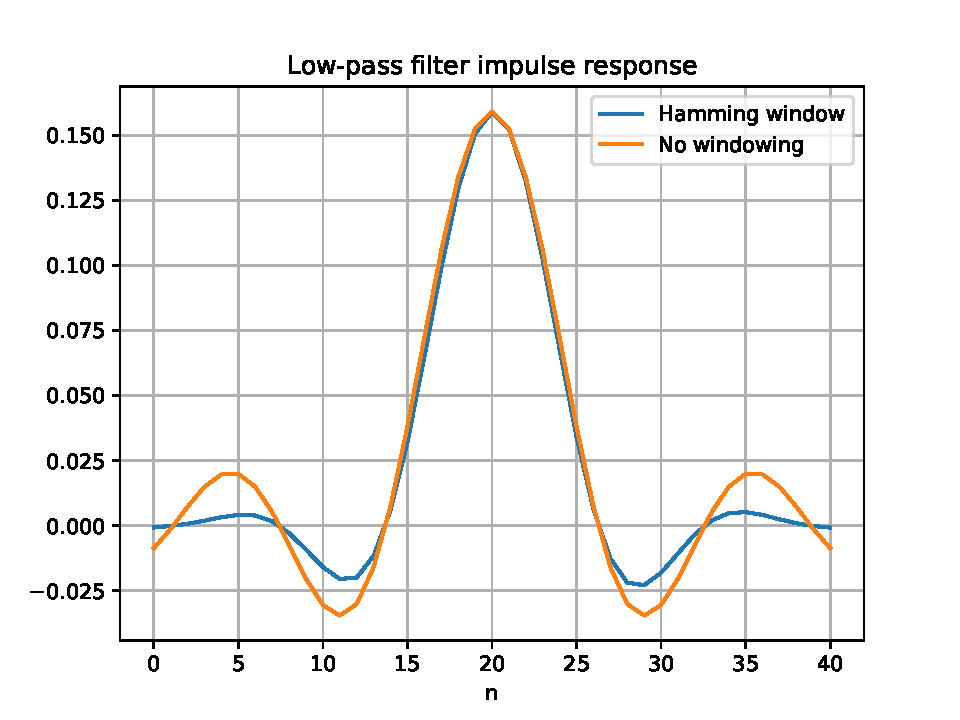
\includegraphics[width=0.5\textwidth]{figures/impulse_response.pdf}
    \caption{Impulse response of the low-pass filter with N=20.}
    \label{fig:low_pass_filter}
\end{figure}

The frequency response of the low-pass filter is determined by filtering cosine waves with increasing frequencies
and calculating the highest amplitude of the output signal.
This is shown for different filter lengths in Figure \ref{fig:cut_off}.
Here, the cut-off frequency is 10 \({rad}/s\).
It can be observed that the steepness of the transition band increases with the filter length.
If no Hamming window is applied, there are ripples in the passband and the stopband.

\begin{figure}[h!]
    \centering
    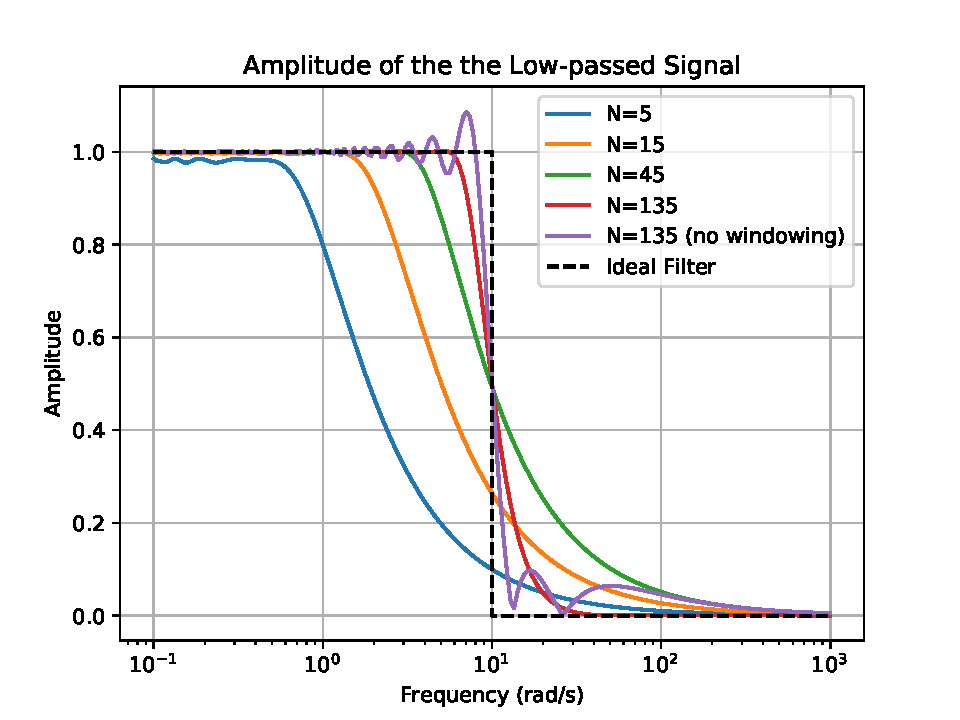
\includegraphics[width=0.5\textwidth]{figures/passband.pdf}
    \caption{Amplitude of the low-passed signal with different filter lengths.}
    \label{fig:cut_off}
\end{figure}

The performance of the low-pass filter highly depends on the implementation of the convolution.
Table \ref{tab:timing_comparison} shows the timing comparison when using fast convolution and convolution in time-domain.
For the given parameters, the fast convolution is on average more than 2.4 times faster then in time-domain.

\begin{table}[h!]
    \centering
    \begin{tabular}{|l|c|c|}
        \hline
                           & \textbf{Fast Convolution} & \textbf{Time-Domain Convolution} \\ \hline
        Average time       & 0.2997 \(s\)              & 0.7241 \(s\)                     \\ \hline
        Standard deviation & 0.0397 \(s\)              & 0.0603 \(s\)                     \\ \hline
        Min time           & 0.2598 \(s\)              & 0.6684 \(s\)                     \\ \hline
        Max time           & 0.5171 \(s\)              & 1.269 \(s\)                      \\ \hline
        Median time        & 0.2864 \(s\)              & 0.715 \(s\)                      \\ \hline
    \end{tabular}
    \caption{Timing comparison for Low-Pass Filter using fast convolution and time-domain convolution. Function length = 20000, Filter length = 50, Number of tests = 200.}
    \label{tab:timing_comparison}
\end{table}

\section{Overall system}

The overall system recreates the transmission of two signals over a common medium using modulation.
On the sender side, the signals are low-pass filtered, modulated and added.
The sum of both modulated signals is then transmitted to the receiver,
where the signal is demodulated and low-pass filtered again.

For testing the overall system, the following signals are used.
The first signal is a sum of cosine waves (Equation 1)
and the second signal is a sawtooth wave (Equation 2).
\begin{equation}
    f_1(t) = 3 + cos(t+1) + 2cos(3t+2) - 5cos(4t-1) + cos(13t)
\end{equation}
\begin{equation}
    f_2(t) = 3 \cdot (t\mod\pi)
\end{equation}
Both signals are sampled 32 times in the interval from 0 to 2\(\pi\).
Each step of the transmission is shown in Figure \ref{fig:overall}, where the left side depicts the operations in time-domain
and the right side in frequency-domain, by showing the magnitude of the first half of the Fourier coefficients.
\begin{figure}[h!]
    \centering
    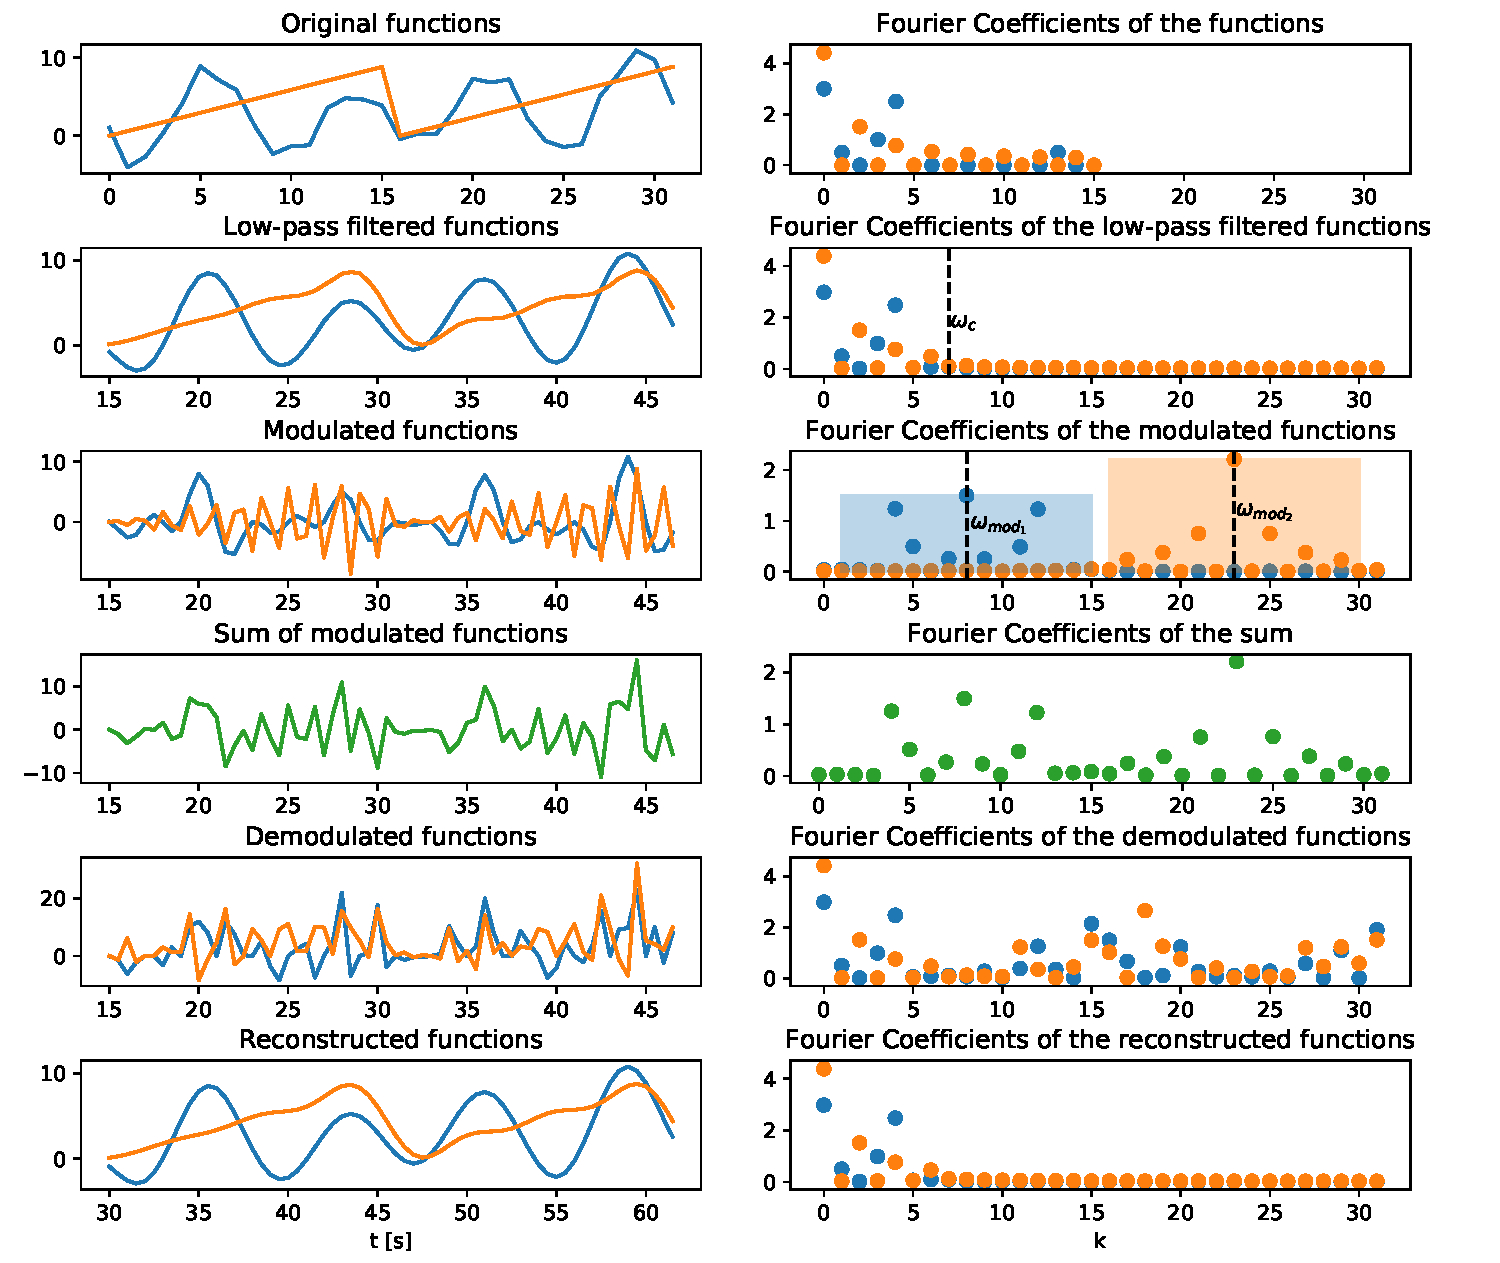
\includegraphics[width=\textwidth]{figures/overall_sampling.pdf}
    \caption{Overall sytsem.}
    \label{fig:overall}
\end{figure}

The cut-off frequency is choosen to be 7 times the base frequency of the cosine wave.
As seen in the second row, the low-pass filter removes the high frequency components.
Then the signals are modulated, so that their frequency bands do not overlap.
After adding, demodulation and low-pass filtering, the reconstructed signals are nearly equal to the original, low-passed signals.

When a overlap of the frequency bands is introduced, the signals cannot be reconstructed properly.
This is shown in Figure \ref{fig:overlap}, where the signals contaian noise of the other signal.
\begin{figure}[h!]
    \centering
    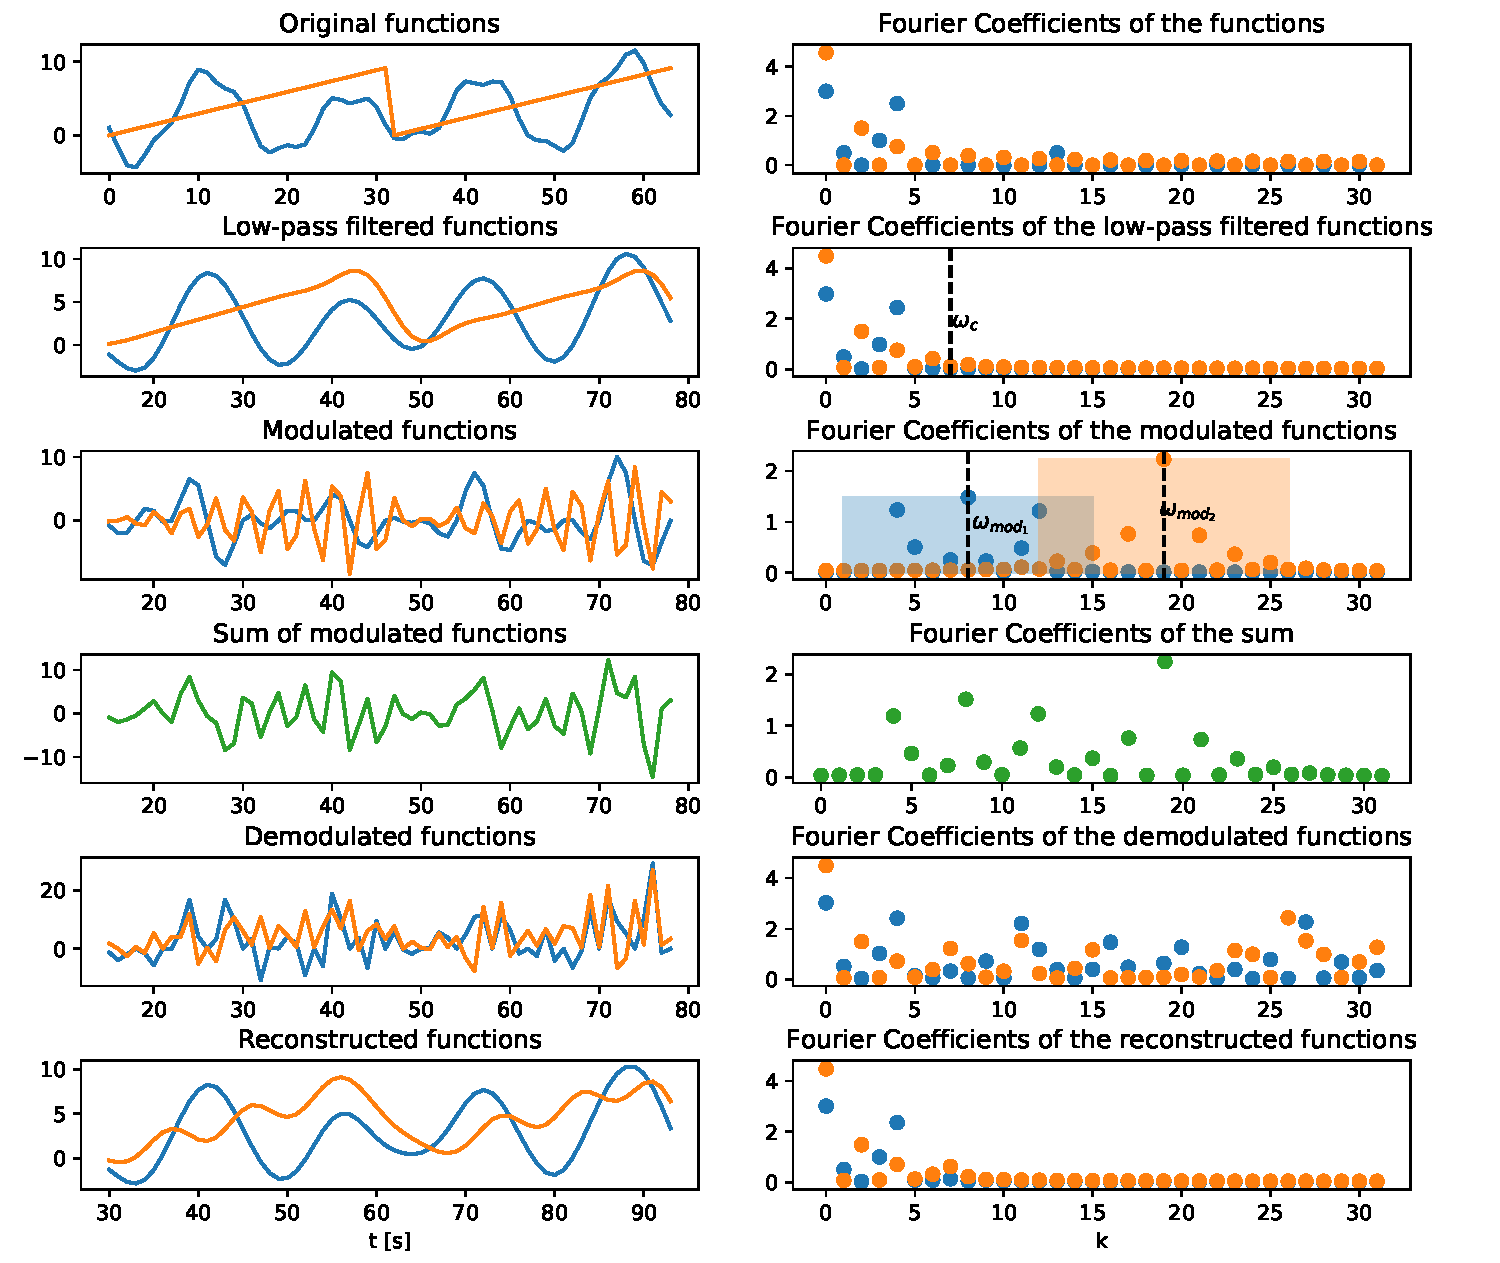
\includegraphics[width=\textwidth]{figures/overall_overlapping.pdf}
    \caption{Overall sytsem with overlapping frequency bands.}
    \label{fig:overlap}
\end{figure}
\end{document}
